\chapter{\label{CMS}The CMS Detector}


The Large Hadron Collider(LHC) is 








The  Large Hadron Collider (LHC), 27 km long, is the largest and most powerful particle accelerator ever manufactured. The protons is accelerated in clockwise and counterclockwise direction to near the speed of light, causing them to collide at four different positions around the ring, as shown in \autoref{fig:my_label_LHC}. At these points, the energy of the collision of the particles is converted to mass and the particles are sprayed in all directions \cite{CMS_1}. The Compact Muon Solenoid (or CMS) detector is located at one of these four collision points. It was designed to observe  new physical phenomena that the LHC may reveal.

%%%%%%%%%%%%%Start from here%%%%5555555555


The CMS acts as a giant high-speed camera, taking 3D "photographs" of particle collisions from all directions up to 40 million times per second. Most of the particles produced by the collision are "unstable" and short-lived, but quickly turn into stable particles that can be detected by the CMS.\cite{CMS_1}-\cite{CMS:2008xjf}.
 CMS is 15 meters in diameter. CMS magnets are the central device on which experiments are built, with a magnetic field of 4 Tesla about $10^6$ times stronger than Earth.\cite{CMS:2008xjf}\cite{CMS_2}.
 \begin{figure}[H]
     \centering
     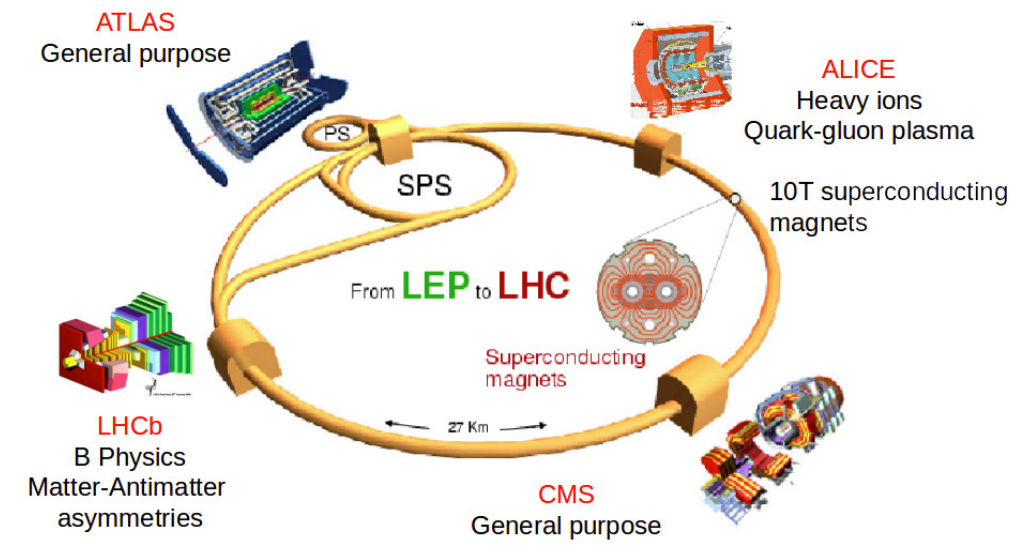
\includegraphics[scale=0.3]{Detector/14__ml.png}
     \caption{LHC}
     \label{fig:my_label_LHC}
 \end{figure}
A magnetic field is used to track the path of a particle to measure its momentum\cite{CMS_1}. The greater the momentum of a particle, the less likely it is that the  path will be curved by a magnetic field. Therefore, following that path gives a measurement of particle momentum. The tracker and calorimeter detectors (ECAL and HCAL) fit snugly inside the magnetic coil, and the muon detector surrounds the magnetic coil and is inserted into a 12-sided iron structure that contains and guides the magnetic field(as can be seen from the \autoref{fig:my_label_detect})\cite{CMS_2} and in \autoref{fig:my_label_CMS}.
\begin{figure}[H]
    \centering
    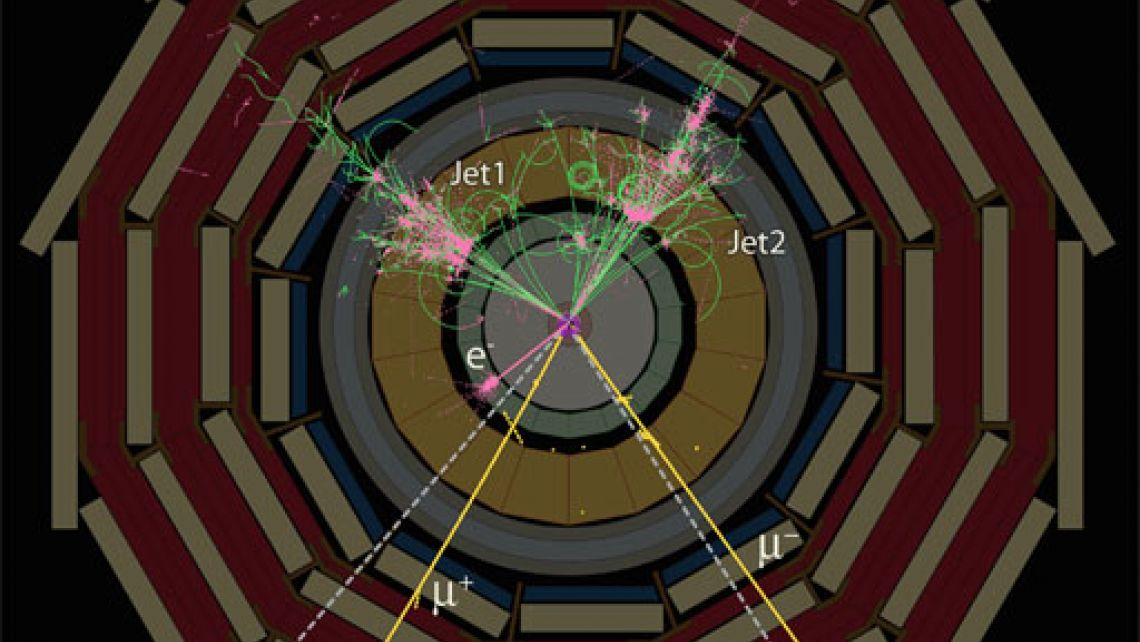
\includegraphics[scale=0.3]{Detector/SusyAny.jpg}
    \caption{This event indicates the formation of  supersymmetric particles. Particle decay  is like requiring an individual CMS layer  to detect the entire range of particles being formed (electrons, muon neutrinos, neutrinos, jets produced by quarks).\cite{CMS_3}}
    \label{fig:my_label_detect}
\end{figure}

\begin{figure}[H]
    \centering
    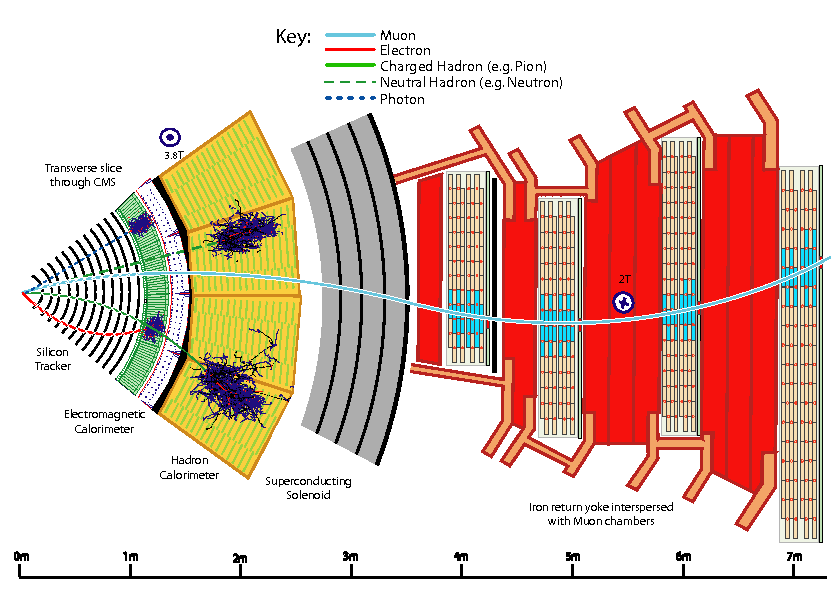
\includegraphics[scale=0.4]{Detector/Figure_001.png}
    \caption{
    Transverse slice of the CMS detector. From the beam interaction zone to the muon detector, a transverse slice of the CMS detector shows unique particle interactions overview. The electron is negatively charged, while the muon and charged pion are positively charged.\cite{CMS_3}}
    \label{fig:my_label_CMS}
\end{figure}

The main function of CMS detector is:
\begin{itemize}
    \item Bending Particles
    \item Identifying tracks
    \item Measuring energy
    \item Detecting muons
\end{itemize}
There are many other use such as medical imagining and etc.\\
A CMS consists of a layer of detector material that captures and measures the energy or momentum of each particle by taking advantage of the various properties of the particle. New particles found in CMS usually quickly transform into an lighter, more stable, better-understood cascade of particles.




% \includemovie{1cm}{1cm}{Figures/detectoroverview.gif}
% \includegraphics{Figures/detectoroverview.gif}
A particle which emerges from the collision, travel outwards will first encounter the tracking system, made of silicon pixels and silicon strip detectors\cite{Sirunyan_2021}. This pixels and strip detectors act as a camera. The detector accurately measure the positions of passing charged particles and allowing physicists to reconstruct their tracks. Charged particles follow spiraling paths in the CMS magnetic field and the curvature of their paths reveal their momenta.\cite{CMS_3}\\
On the way out of the tracker, the particles pass through 10 layers of a 130 cm silicon strip detector. This tracker silicon strip detector consists of four inner  layers (TIBs) assembled into a shell with two internal end caps (TIDs), each with three small discs. The outer barrel (TOB) consists of six concentric layers (see \autoref{fig:my_label_Concentric}). Finally, the two end caps (TECs) close  the tracker. Each has a silicon module designed to be different depending on its position in the detector. This part of the tracker contains 15,200  sensitive modules and a total of 10 million detector strips read by 80,000 microelectronic chips. Each module consists of three elements: sensors, mechanical support structure and electronics. These silicon are very suited to receive many particles in a small space due to their fast response and good spatial resolution. The small amount of charge generated after knocking of electron from atoms get amplified by APV25 chips, allows us to reconstruct its path.
\begin{figure}[H]
    \centering
    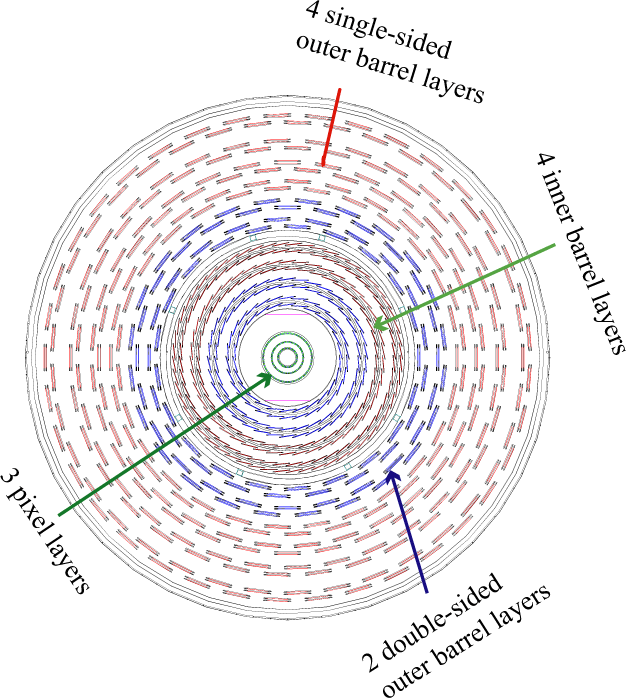
\includegraphics[scale=0.3]{Detector/Barrel.png}
    \caption{CMS Tracker layer shown in perpendicular to the beam\cite{CMS_6}}
    \label{fig:my_label_Concentric}
\end{figure}

The  next layer of the detector,the calorimeter, measures the energy of the emitted particles. Electrons, photons, and jets (particulate sprays produced by quarks) are all  stopped by a calorimeter so that their energy can be measured. The first calorimeter layer is designed to measure electron and photon energies  with high accuracy. As all these particles interact electromagnetically and are therefore called an electromagnetic calorimeter(ECAL)\cite{CMS_4}.

Particles that interact through the strong force hadron store most of their energy in the next layer, the hadron calorimeter (HCAL). The only known particles that penetrate beyond  HCAL are  weakly interacting particles such as muons and neutrinos. Muons are charged particles and are further tracked by muon chamber detectors. Their momentum is also measured from the curvature of the path of the CMS magnetic field. However, neutrinos are neutral and have little interaction, so they avoid detection. We can determine where those particles were by adding  the momentums of all the detected particles and assigning the lost momentum to the neutrinos.

% \section{TRIGGERING AND DATA ACQUISITION}
We need a "trigger" to select  potentially interesting events (such as the Higgs boson) from a larger dataset generated after a proton-proton interaction collision. These triggers help reduce the rate to just a few hundred "events" per second. These events can be sampled and stored on your computer's hard drive for later analysis.\cite{CMS_5}. At the end, We are only left with only the collision events that might teach us something new about physics.
% When CMS is performing at its peak, about one billion proton-proton interactions will take place every second inside the detector. There is no way that data from all these events could be read out, and even if they could, most would be less likely to reveal new phenomena; they might be low-energy glancing collisions for instance, rather than energetic, head-on interactions.We therefore need a “trigger” that can select the potentially interesting events, such as those which will produce the Higgs particle, and reduce the rate to just a few hundred “events” per second, which can be read out and stored on computer disk for subsequent analysis.\\

% However, with groups of protons colliding 40 million times per second there are only ever 25 nanoseconds (25 billionths of a second) before the next lot arrive. New waves of particles are being generated before those from the last event have even left the detector! The solution is to store the data in pipelines that can retain and process information from many interactions at the same time. To not confuse particles from two different events, the detectors must have very good time resolution and the signals from the millions of electronic channels must be synchronised so that they can all be identified as being from the same event.\\
% Level 1 of the trigger is an extremely fast and wholly automatic process that looks for simple signs of interesting physics, e.g. particles with a large amount of energy or in unusual combinations. This is like a reader simply scanning the headlines of a newspaper to see if anything catches their eye. This way we select the best 100,000 events or “issues” each second from the billion available. For the next test, the higher level trigger, we assimilate and synchronise information from different parts of the detector to recreate the entire event - like collating the different pages to form the full newspaper - and send it to a farm of more than 1000 standard computers.


% \url{https://cms.cern/detector/triggering-and-data-acquisition}


% \section{SILICON STRIPS}
% https://cms.cern/detector/identifying-tracks/silicon-strips



% After the pixels and on their way out of the tracker, particles pass through ten layers of silicon strip detectors, reaching out to a radius of 130 centimetres.
% The tracker silicon strip detector consists of four inner barrel (TIB) layers assembled in shells with two inner endcaps (TID), each composed of three small discs. The outer barrel (TOB) consists of six concentric layers. Finally two endcaps (TEC) close off the tracker. Each has silicon modules designed differently for its place within the detector. This part of the tracker contains 15,200 highly sensitive modules with a total of 10 million detector strips read by 80,000.  Each module consists of three elements: a set of sensors, its mechanical support structure and readout electronics. \\
% Silicon sensors are highly suited to receive many particles in a small space due to their fast response and good spatial resolution. microelectronic chips. Each module consists of three elements: a set of sensors, its mechanical support structure and readout electronics. \\
% Silicon sensors are highly suited to receive many particles in a small space due to their fast response and good spatial resolution. The silicon detectors work in much the same way as the pixels: as a charged particle crosses the material it knocks electron from atoms and within the applied electric field these move giving a very small pulse of current lasting a few nanoseconds. This small amount of charge is then amplified by APV25 chips, giving us “hits” when a particle passes, allowing us to reconstruct its path.

% Due to the nature of their job, the tracker and its electronics are pummeled by radiation but they are designed to withstand it. To minimise disorder in the silicon this part of the detector is kept at -20oC, to “freeze” any damage and prevent it from perpetuating.

% The charge on each microstrip is read out and amplified by an Analogue Pipeline Voltage (APV25) chip. Four or six such chips are housed within a “hybrid”, which also contains electronics to monitor key sensor information, such as temperature, and provide timing information in order to match “hits” with collisions. The APV25 stores the signals in a memory for several microseconds and then processes them before sending to a laser to be converted into infrared pulses. These are then transmitted over a 100m fibre optic cable for analysis in a radiation-free environment. The tracker uses 40,000 such fibre optic links providing a low power, lightweight way of transporting the signal. Much of the technology behind the tracker electronics came from innovation in collaboration with industry. \\
% \section{SILICON PIXELS}

% https://cms.cern/detector/identifying-tracks/silicon-pixels

% \section{TRACKING}
% https://cms.cern/detector/identifying-tracks

% The pixel detector, though about the size of a shoebox, contains 65 million pixels, allowing it to track the paths of particles emerging from the collision with extreme accuracy. Each layer is spilt into segments like tiny kitchen tiles, each a little silicon sensor, 100µm by 150µm, about two hairs widths. When a charged particle passes through it gives enough energy for electrons to be ejected from the silicon atoms, creating electron-hole pairs. Each pixel uses an electric current to collect these charges on the surface as a small electric signal. A electronic silicon chip, one for each tile is attached, using an almost microscopic spot of solder using the so-called bump bonding technique, which amplifies the signal.Knowing which pixels have been touched allows us to deduce the particle's trajectory. And because the detector is made of 2D tiles, rather than strips, and has a number of layers, we can create a three-dimensional picture. Because there are 65 million channels, the power for each pixel must be kept to a minimum. Even with each only generating around 50 microwatts, the total power output is around the same as the energy produced by a hot plate. So as not to overheat the detector, the pixels are mounted on cooling tubes.\\
% % \section{MEASURING ENERGY}
% https://cms.cern/detector/measuring-energy
% Electromagnetic calorimeters (ECALs) are two inner layers that measure their energy by completely stopping electrons and photons. Hadrons, a composite particle of quarks and gluons, pass through the ECAL and are blocked by an outer layer called the hadron calorimeter (HCAL). A photodetector specifically designed to work in high magnetic fields is also glued to the back of each crystal to capture scintillation light and convert it into an electrical signal.
 
% \section{ENERGY OF ELECTRONS AND PHOTONS (ECAL)}
% https://cms.cern/detector/measuring-energy/energy-electrons-and-photons-ecal\\
% CMS must find the energies of emerging particles. Of particular interest are electrons and photons, because of their use in finding the Higgs boson and other new physics.

% The particles are measured using an electromagnetic calorimeter (ECAL). But to find them with the necessary precision in the very strict conditions of the LHC - a high magnetic field, high levels of radiation and only 25 nanoseconds between collisions - required very particular detector materials.\\ 
% Lead tungstate crystal is made primarily of metal and is heavier than stainless steel, but with a touch of oxygen in this crystalline form it is highly transparent and “ scintillates ” when electrons and photons pass through it. This means it produces light in proportion to the particle’s energy. These high-density crystals produce light in fast, short, well-defined photon bursts that allow for a precise, fast and fairly compact detector.

% Photodetectors that have been especially designed to work within the high magnetic field, are also glued onto the back of each of the crystals to detect the scintillation light and convert it to an electrical signal that is amplified and sent for analysis.

% The ECAL, made up of a barrel section and two ”endcaps”, forms a layer between the tracker and the HCAL. The cylindrical “barrel” consists of 61,200 crystals formed into 36 “supermodules”, each weighing around three tonnes and containing 1700 crystals. The flat ECAL endcaps seal off the barrel at either end and are made up of almost 15,000 further crystals.

% For extra spatial precision, the ECAL also contains Preshower detectors that sit in front of the endcaps. These allow CMS to distinguish between single high-energy photons (often signs of exciting physics) and the less interesting close pairs of low-energy photons.
% The CMS ECAL…

% crystals each weigh 1.5kg but with a volume roughly equal to that of a small coffee cup,
% contains nearly 80,000 such crystals, each of which took two days to grow.

% https://cms.cern/detector/measuring-energy/energy-hadrons-hcal\\

% https://cms.cern/detector/detecting-muons\\
% https://cms.cern/detector/computing-grid\\
To meet this challenge, the vast amount of data obtained from the CMS needs to be analyzed, and LHC has adopted a new computing system, a distributed computing and data storage infrastructure called the Worldwide LHC Computing Grid (WLCG). doing. The grid works together with tens of thousands of standard PCs around the world to provide far more processing power than  a single supercomputer can achieve, giving  thousands of scientists around the world access to data. \cite{CMS_7}.

% The “Tier 0” centre at CERN first reconstructs the full collision events and analysts start to look for patterns; but the data has a long way to go yet. Once CERN has made a primary backup of the data it is then sent to large “Tier 1” computer centres in seven locations around the world: in France, Germany, Italy, Spain, Taiwan, the UK and the US. Here events are reconstructed again, using information from the experiment to improve calculations using refined calibration constants.

% Tier 1 starts to interpret and make sense of the particle events and collate the results to see patterns emerging. Meanwhile each sends the most complex events to a number of “Tier 2” facilities, which total around 40, for further specific analysis tasks. In this way information braches out from each tier across the world so that, on a local level.
% , physicists and students whether in Rio de Janeiro or Oxford, can study CMS data from their own computer, updated on a regular basis by the LHC Computing Grid.
 Charged particle trajectories are measured by the silicon pixel and strip sub detectors\cite{Palichik:2018wwn}, covering 0 <$\phi$ <2$\pi$ in azimuth and $|\eta|$ < 2.5, where the pseudo rapidity $\eta$ is defined as 
 \begin{equation*}
     \eta = -ln[\tan \theta/2],
 \end{equation*}
 
 with $\theta$ being the polar angle of the trajectory of the particle with respect to the
 counterclockwise beam direction, as shown in the \autoref{fig:my_label_CMS_COOR}. Within the field
volume, the silicon detectors are surrounded by a crystal electromagnetic calorimeter and a brass/scintillator hadron calorimeter that provide high resolution energy measurement of photons, electrons and hadronic jets.

\begin{figure}[H]
    \centering
    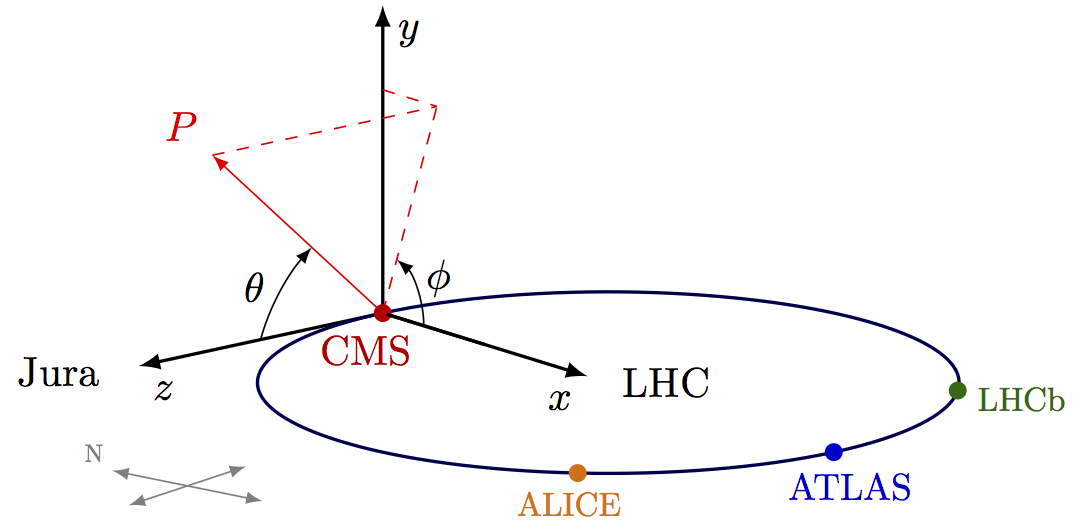
\includegraphics{figure_1/cms_coordinate_system.png}
    \caption{The coordinate system used to measure the momenta of the particle.}
    \label{fig:my_label_CMS_COOR}
\end{figure}


% \textbf{Complte this part in 1500- 2000 words}
% The Compact Muon Solenoid (CMS) is a particle detector built to study pp collisions at the LHC.
% The detector has a diameter of 15 m and a length of 21.6 m. The key feature of the detector is
% its large superconducting solenoid with an internal diameter of 6m that creates a magnetic field
% of 3.8 T. The magnetic field helps to bend the trajectories of charged particles in order to identify
% their momentum and charge. Fig 1.3 shows a transverse view of the detector.
% The detector is built hermetically around the beam pipe (where pp collisions take place) and has
% several different modules specialized in identifying certain types of particles. Closest to the beam
% pipe are the silicon pixel and strip detectors, which help in identifying charged particle tracks.
% Surrounding this is the Electromagnetic Calorimeter (ECAL), which is made up of scintillating
% lead-tungstate crystals and helps to identify energy deposits from photons and electrons. The
% Hadron Calorimeter (HCAL) is a sampling calorimeter built from brass and a scintillator and helps
% to identify energy deposits from charged and neutral hadrons. The pixel and strip trackers, ECAL
% and the HCAL are enclosed within the solenoid (magnetic) volume. Outside the magnet are the
% muon chambers which are gas ionization chambers and are used to identify muons. These muon
% chambers are embedded in steel return yokes of the magnet. Muons can travel several metres
% without interacting. This is the reason why muon detectors are placed at the outer edge of the



% About LHC
% The Large Hadron Collider (LHC) is the world’s largest and most powerful particle accelerator. The LHC consists of a 27-kilometer ring of superconducting magnets with a number of accelerating structures to boost the energy of the particles along the way. Inside the accelerator, two high-energy particle beams travel at close to the speed of light before they are made to collide. The beams travel in opposite directions in separate beam pipes – two tubes kept at ultrahigh vacuum. They are guided around the accelerator ring by a strong magnetic field maintained by superconducting electromagnets. The electromagnets are built from coils of special electric cable that operates in a superconducting state, efficiently conducting electricity without resistance or loss of energy. This requires chilling the magnets to ‑271.3°C. For this reason, much of the accelerator is connected to a distribution system of liquid helium, which cools the magnets, as well as to other supply services. Thousands of magnets of different varieties and sizes are used to direct the beams around the accelerator. These include 1232 dipole magnets 15 metres in length which bend the beams, and 392 quadrupole magnets, each 5–7 metres long, which focus the beams. 
% protons for beams in 27-kilometre ring come from a single bottle of hydrogen gas, replaced only twice per year to ensure that it is running at the correct pressure.
% How to accelerate protons
% In the first part of the accelerator, an electric field strips hydrogen atoms (consisting of one proton and one electron) of their electrons. Electric fields along the accelerator switch from positive to negative at a given frequency, pulling charged particles forwards along the accelerator. CERN engineers control the frequency of the change to ensure the particles accelerate not in a continuous stream, but in closely spaced “bunches”.

% Radiofrequency (RF) cavities
% These are specially designed metallic chambers, spaced at intervals along the accelerator – are shaped to resonate at specific frequencies, allowing radio waves to interact with passing particle bunches. Each time a beam passes the electric field in an RF cavity, some of the energy from the radio waves is transferred to the particles, nudging them forwards.It’s important that the particles do not collide with gas molecules on their journey through the accelerator, so the beam is contained in an ultrahigh vacuum inside a metal pipe – the beam pipe.

% Various types of magnet
% These serve different functions around a circular accelerator. Dipole magnets, for example, bend the path of a beam of particles that would otherwise travel in a straight line. The more energy a particle has, the greater the magnetic field needed to bend its path. Quadrupole magnets act likes lenses to focus a beam, gathering the particles closer together. 


% Energies Units 
% Energy has many units in physics: joules, calories, and kilowatt hours are all units of energy used in different contexts. Only the joule is an International System (SI) unit, but all of them are related by conversion factors. In particle physics, the unit that is most frequently used for energy is the electronvolt (eV) and its derivatives keV (10^3 eV), MeV (10^6 eV), GeV (10^9 eV) and TeV (10^12 eV). The electronvolt is a convenient unit because, in absolute terms, the energies that particle physicists deal with are very small. If we take the LHC as an example, the design value of the total collision energy is 14 TeV

% The definition of the electronvolt comes from the simple insight that a single electron accelerated by a potential difference of 1 volt will have a discrete amount of energy (measured in joules), E=qV where q is the charge on the electron in coulombs and V is the potential difference in volts. Hence 1 eV = (1.602 x 10–19 C) x (1 V) = 1.602 x 10–19 J.

% What is an accelerator?
% An accelerator propels charged particles, such as protons or electrons, at high speeds, close to the speed of light. They are then smashed either onto a target or against other particles circulating in the opposite direction. By studying these collisions, physicists are able to probe the world of the infinitely small.

 
% The Large Hadron Collider is the most powerful accelerator in the world. It boosts particles, such as protons, which form all the matter we know. Accelerated to a speed close to that of light, they collide with other protons. These collisions produce massive particles, such as the Higgs boson or the top quark. By measuring their properties, scientists increase our understanding of matter and of the origins of the Universe. These massive particles only last in the blink of an eye, and cannot be observed directly. Almost immediately they transform (or decay) into lighter particles, which in turn also decay. The particles emerging from the successive links in this decay chain are identified in the layers of the detector.



% How an accelerator works
% Their job is to speed up and increase the energy of a beam of particles by generating electric fields that accelerate the particles, and magnetic fields that steer and focus them. 
% Accelerators use electromagnetic fields to accelerate and steer particles. Radiofrequency cavities boost the particle beams, while magnets focus the beams and bend their trajectory.
% In a circular accelerator, the particles repeat the same circuit for as long as necessary, getting an energy boost at each turn. In theory, the energy could be increased over and over again. However, the more energy the particles have, the more powerful the magnetic fields have to be to keep them in their circular orbit.
% A linear accelerator, on the contrary, is exclusively formed of accelerating structures since the particles do not need to be deflected, but they only benefit from a single acceleration pass. In this case, increasing the energy means increasing the length of the accelerator.
% As physicists have been explored higher and higher energies, accelerators have become larger and larger: the size of an accelerator is a compromise between energy, the radius of curvature (if it’s circular), the feasibility and the cost.
% Colliders are accelerators that generate head-on collisions between particles. Thanks to this technique, the collision energy is higher because the energy of the two particles is added together.
% The Large Hadron Collider is the largest and most powerful collider in the world. It boosts the particles in a loop 27 kilometres in circumference at an energy of 6.5 TeV (teraelectronvolts), generating collisions at an energy of 13 TeV.
% What are the characteristics of an accelerator?
% The type of particles, the energy of the collisions and the luminosity are among the important characteristics of an accelerator. An accelerator can circulate a lot of different particles, provided that they have an electric charge so that they can be accelerated with an electromagnetic field. The CERN accelerator complex accelerates protons, but also nuclei of ionized atoms (ions), such as the nuclei of lead, argon or xenon atoms. Some LHC runs are thus dedicated to lead-ion collisions. The ISOLDE facility accelerates beams of exotic nuclei for nuclear physics studies. The energy of a particle is measured in electronvolts. One electronvolt is the energy gained by an electron that accelerates through a one-volt electrical field. As they race around the LHC, the protons acquire an energy of 6.5 million million electronvolts, known as 6.5 tera-electronvolts or TeV. It is the highest energy reached by an accelerator, but in everyday terms, this is a ridiculously tiny energy; roughly the energy of a safety pin dropped from a height of just two centimetres. But an accelerator concentrates that energy at the infinitesimal scale to obtain very high concentrations of energy close to those that existed just after the Big Bang.
% Luminosity is a key indicator of an accelerator’s performance: it indicates the number of potential collisions per surface unit over a given period of time. The instantaneous luminosity is expressed in cm-2s-1 and the integrated luminosity, corresponding to the number of collisions that can occur over a given period, is measured in inverse femtobarn. One inverse femtobarn corresponds to 100 million millions (potential) collisions.
% What type of accelerators are at CERN?
% CERN operates a complex of eight accelerators and two decelerators. These accelerators supply experiments or are used as injectors, accelerating particles for larger accelerators. Some, such as the Proton Synchrotron (PS) or Super Proton Synchrotron (SPS) do both at once, preparing particles for experiments that they supply directly and injecting into larger accelerators.
% The Large Hadron Collider is supplied with protons by a chain of four accelerators that boost the particles and divide them into bunches.
 
% CERN’s accelerator complex

% The accelerator complex at CERN is a succession of machines that accelerate particles to increasingly higher energies. Each machine boosts the energy of a beam of particles before injecting it into the next machine in the sequence. In the Large Hadron Collider (LHC) – the last element in this chain – particle beams are accelerated up to the record energy of 6.5 TeV per beam.
 
% Linear accelerator 4 (Linac4) became the source of proton beams for the CERN accelerator complex in 2020. It accelerates negative hydrogen ions (H-, consisting of a hydrogen atom with an additional electron) to 160 MeV to prepare them to enter the Proton Synchrotron Booster (PSB). The ions are stripped of their two electrons during injection from Linac4 into the PSB, leaving only protons. These are accelerated to 2 GeV for injection into the Proton Synchrotron (PS), which pushes the beam up to 26 GeV. Protons are then sent to the Super Proton Synchrotron (SPS), where they are accelerated up to 450 GeV.

% The protons are finally transferred to the two beam pipes of the LHC. The beam in one pipe circulates clockwise while the beam in the other pipe circulates anticlockwise. It takes 4 minutes and 20 seconds to fill each LHC ring, and 20 minutes for the protons to reach their maximum energy of 6.5 TeV. Beams circulate for many hours inside the LHC beam pipes under normal operating conditions. The two beams are brought into collision inside four detectors – ALICE, ATLAS, CMS and LHCb – where the total energy at the collision point is equal to 13 TeV.
% Protons are not the only particles accelerated in the LHC. Lead ions for the LHC start from a source of vaporised lead and enter Linac3 before being collected and accelerated in the Low Energy Ion Ring (LEIR). They then follow the same route to maximum energy as the protons.


% Luminosity gives a measure of how many collisions are happening in a particle accelerator, so why don’t we just say collision rate?
% Luminosity gives a measure of how many collisions are happening in a particle accelerator, so we’re often asked why we don’t just say collision rate. It’s a very reasonable question. The answer is because luminosity isn’t strictly speaking the collision rate: it measures how many particles we’re able to squeeze through a given space in a given time. That doesn’t mean that those particles will all collide, but the more we can squeeze into a given space, the more likely they are to collide.
% The best place to start is with what physicists refer to as a cross-section. Usually, a cross-section is a measure of the size of something. For example, a barn door has a bigger cross-section – it covers a larger area – than a cat flap. In particle physics, a cross-section is a measure of the probability of something happening, and it’s measured in units called…. barns. In reality, a barn is a huge cross-section and most processes have cross-sections measured in tiny fractions of a barn.
% When protons collide in the LHC, many things can happen: the protons can just glance off each other, or they can collide more violently producing any of a range of new particles. Each of these processes has its own cross-section. The cross-section for the production of a Higgs particle, for example, is very small at the scale of nanobarns – billionths of a barn  – which means that Higgs particles, if they exist, will be produced very rarely.
% When looking for something that rare, the more collisions you have, the more likely it is that the rare thing will happen, and that’s why particle physicists care so much about luminosity. It works a bit like this: if you multiply the luminosity of the beam by the cross-section for any process, such as Higgs production, you get the rate at which you can expect that process to happen. If you multiply the luminosity by the sum of the cross-sections for all possible processes, you get the total number of collisions.
% To help figure out the different ways that luminosity contributes to the collision rate, think of rolling marbles from opposite ends of a corridor. If you’ve just got one person at each end of the corridor, the chances they’ll get their marbles to collide are small: the luminosity is pretty low. But put lots of people at each end and the luminosity goes up. Similarly, if you increase the cross-section by rolling footballs down the corridor, the luminosity remains the same, but since a football has a bigger cross-section than a marble, the number of collisions goes up. It’s not a perfect analogy, but I hope you get the idea.
% The LHC’s design luminosity is 1034 per square centimetre per second. That’s a big number, and although we can’t say exactly how many collisions it equates to, we can say that and it’s around 600 million collisions per second on average. When the LHC run ended in 2010, the luminosity was around 2×1032 per square centimetre per second, giving a few million proton collisions per second.
% The other way that physicists use luminosity is to add it all up, or integrate it. If you do that, you get a measure of the total number of collisions that have happened. So, for example, the integrated luminosity recorded by the ATLAS and CMS experiments in 2010 was around 45 inverse picobarns, which translates to over 3000 billion collisions recorded.  And what about the Higgs particle? With the peak luminosity reached by the LHC last year, we might have expected Higgs particles to be produced at the rate of a handful a day, which is not yet enough for us to see a signal above the background from known and well-understood physics. To claim a discovery, physicists need to see a statistically significant excess over and above what they expect to see from known physics, and they measure the degree of significance using a quantity called a standard deviation, or sigma for short
% Restarting the LHC: Why 13 Tev?
% The LHC was designed to run at a maximum collision energy of 14 TeV, so why has CERN decided to start the second run at a lower energy?
% The Large Hadron Collider (LHC) is scheduled to restart for physics early in 2015 after two years of maintenance and upgrading. The collision energy at restart will be 13 TeV, a significant increase over the initial three-year LHC run, which began with a collision energy of 7 TeV, rising to 8 TeV. But the LHC was designed to run at a maximum collision energy of 14 TeV, so why has CERN decided to start the second run at a lower energy?
% The decision to begin the LHC’s second run at 13 TeV has been taken in order to optimise the delivery of particle collisions for physics research, and thereby speed the route to potential new physics. It is based on the properties of the 1232 superconducting dipole magnets that guide the beams around the LHC’s 27-kilometre ring. The higher the beam energy, the higher the magnetic field needed to maintain a constant orbit, and the higher the electric current flowing in the magnet’s superconducting coils.
% At LHC beam energies, the electric currents are extremely high, up to 12,000 Amperes, and superconducting cables have to be used. Superconductivity is a low-temperature phenomenon, so the coils have to be kept very cold, just 1.9 degrees above absolute zero to be precise, or about -271°C. Even a tiny amount of energy released into the magnet for any reason can warm the coils up, stopping them from superconducting. When this happens, the current has to be safely extracted in a very short time. This is called a quench, and just one millijoule – the energy deposited by a 1-centime euro coin falling from 5 cm – is enough to provoke one. Magnet protection in case of quenches is a crucial part of the design of the LHC’s magnetic system.  
% When a new superconducting magnet is qualified for use, it needs to be trained. That involves steadily increasing the current until the magnet quenches, then starting again. At first, the quenches may occur at relatively low current, but over time, as the components of the magnet settle in, the current increases until the magnet can be operated routinely at its nominal current. If a new training cycle is started after an extended period during which the magnet is warm, the magnet usually restarts training at a value that is higher than first quench in the first training cycle but lower than the maximum previously reached. In other words, the magnet’s ‘memory’ is usually less than 100%.
% Before the LHC started operation, all of its magnets were trained up to a current equivalent to a collision energy of over 14 TeV. Tests with individual magnets, along with hardware commissioning tests in 2008, have shown that for some dipole magnets the memory is slightly lower than expected, demanding a larger number of quenches to reach nominal field. However, retraining these magnets to 13 TeV should require only a short period of time, whereas retraining to 14 TeV would take longer, taking time away from physics research. That’s why the best way to get to new results quickly, at an energy considerably higher than ever achieved before, is to start operation at 13 TeV. A decision on when to go higher will be taken at a later date in the LHC’s second run..
 
% Interesting:
% https://home.cern/science/accelerators/accelerator-complex/panoramas
% Accelerating: Radiofrequency cavities
% To accelerate particles, the accelerators are fitted with metallic chambers containing an electromagnetic field known as radiofrequency (RF) cavities. Charged particles injected into this field receive an electrical impulse that accelerates them. In the Large Hadron Collider (LHC), 16 RF cavities are housed in four cylindrical refrigerators called cryomodules, which enable them to work in a superconducting state. Each cavity is driven by a high-power klystron, which is a tube containing electron beams. The electron beams are intensity-modulated to a frequency of 400 MHz, or 400 million oscillations per second. A rectangular pipe of conducting metal called a waveguide directs energy to the cavity. The cavity’s shape has been specifically designed to achieve resonance and the build up in intensity of the electromagnetic waves. Each cavity can reach a maximum voltage of 2 megavolts (MV), corresponding to 16 MV per beam. The LHC’s RF cavities bring the 450 GeV energy of the particles (1 GeV = 1 billion electronvolts) to 6.5 TeV (1 TeV = 1 million million electronvolts) - more than 14 times their injection energy. The maximum energy is reached in around 20 minutes with the bunches having passed through the RF cavities more than 10 million times. The field in an RF cavity is made to oscillate (switch direction) at a given frequency, so timing the arrival of particles is important. In the LHC, each RF cavity is tuned to oscillate at 400 MHz. When the beam has reached the required energy, an ideally timed proton with exactly the right energy will not be accelerated. By contrast, protons with slightly different energies arriving earlier or later will be accelerated or decelerated so that they stay close to the desired energy. In this way, the particle beam is sorted into packs of protons called "bunches". Aside from these accelerating cavities, CERN is developing “crab” cavities for the LHC’s successor, the High-Luminosity LHC. The purpose of these crab cavities is to give a transverse momentum to steer the particles as they approach the collision point.
% How a detector works
% Accelerators at CERN boost particles to high energies before they are made to collide inside detectors. The detectors gather clues about the particles – including their speed, mass and charge – from which physicists can work out a particle's identity. The process requires accelerators, powerful electromagnets, and layer upon layer of complex subdetectors.
% Particles produced in collisions normally travel in straight lines, but in the presence of a magnetic field their paths become curved. Electromagnets around particle detectors generate magnetic fields to exploit this effect. Physicists can calculate the momentum of a particle – a clue to its identity – from the curvature of its path: particles with high momentum travel in almost straight lines, whereas those with very low momentum move forward in tight spirals inside the detector.
% Modern particle detectors consist of layers of subdetectors, each designed to look for particular properties, or specific types of particle. Tracking devices reveal the path of a particle; calorimeters stop, absorb and measure a particle’s energy; and particle-identification detectors use a range of techniques to pin down a particle's identity.
% Tracking devices
% Tracking devices reveal the paths of electrically charged particles as they pass through and interact with suitable substances. Most tracking devices do not make particle tracks directly visible, but record tiny electrical signals that particles trigger as they move through the device. A computer program then reconstructs the recorded patterns of tracks.
% One type of particle, the muon, interacts very little with matter – it can travel through metres of dense material before being stopped. Muons, therefore, pass easily through the inner layers of a detector, which is why muon chambers – tracking devices specialized in detecting muons – usually make up the outermost layer of a detector.

% Calorimeters
% A calorimeter measures the energy a particle loses as it passes through. It is usually designed to stop entirely or “absorb” most of the particles coming from a collision, forcing them to deposit all of their energy within the detector, thus measuring their full energy. Calorimeters have to perform two different tasks at the same time – stopping particles and measuring energy loss – so they usually consist of layers of different materials: a “passive” or “absorbing” high-density material – for example, lead – interleaved with an “active” medium such as plastic scintillators or liquid argon.
% Electromagnetic calorimeters measure the energy of electrons and photons as they interact with the electrically charged particles in matter. Hadronic calorimeters sample the energy of hadrons (particles containing quarks, such as protons and neutrons) as they interact with atomic nuclei. Calorimeters can stop most known particles except muons and neutrinos.

% Particle-identification detectors
% In addition to measuring a particle's momentum in tracking devices and its energy in calorimeters, physicists have further methods of narrowing down its identity. These methods all rely on measuring a particle's velocity, since this, in combination with the momentum measured in the tracking devices, helps to calculate a particle's mass and therefore its identity.
% Velocity can be measured using several methods. The simplest is to measure how much time it takes for a particle to travel a certain distance, using precise time-of-flight detectors. Another method looks at how much a particle ionises the matter that it passes through, as this is velocity-dependent and can be measured by tracking devices.
% If a charged particle travels faster than light through a given medium, it emits Cherenkov radiation at an angle that depends on its velocity. Alternatively, when a particle crosses the boundary between two electrical insulators with different resistances to electric currents, it emits transition radiation, the energy of which depends on the particle's velocity.
% Collating all these clues from different parts of the detector, physicists build up a snapshot of what was in the detector at the moment of a collision. The next step is to scour the collisions for unusual particles, or for results that do not fit current theories.
% Insertion magnets
% When the particle beams enter the detectors, insertion magnets take over. Particles must be squeezed closer together before they enter a detector so that they collide with particles coming from the opposite direction. Three quadrupoles are used to create a system called an inner triplet. There are eight inner triplets, two of which are located at each of the four large LHC detectors, ALICE, ATLAS, CMS and LHCb. Inner triplets tighten the beam, making it 12.5 times narrower – from 0.2 millimetres down to 16 micrometres across.
% After the beams collide in the detector, enormous magnets aid the measurement of particles. For example, physicists look at how charged particles bend in the magnetic field to determine their identity. Charged particles are deflected by the magnetic field in the detector, and their momentum can be calculated from the amount of deflection.
% After colliding, the particle beams are separated again by dipole magnets. Other magnets minimize the spread of the particles from the collisions. When it is time to dispose of the particles, they are deflected from the LHC along a straight line towards the beam dump. A "dilution" magnet reduces the beam intensity by a factor of 100,000 before the beam collides with a block of concrete and graphite composite for its final stop.
% Insertion magnets are also responsible for beam cleaning, which ensures that stray particles do not come in contact with the LHC’s most sensitive components.
\setcounter{equation}{0}
\setcounter{table}{0}
\setcounter{figure}{0}
%\baselineskip 24pt


    


